\documentclass[a4paper]{report}

% Настройка русского шрифта
\usepackage[T2A]{fontenc}
\usepackage[utf8]{inputenc}
\usepackage[english, russian]{babel}

% Отключение нумерации страниц
\usepackage{nopageno}

% Для операций по модулю
\usepackage{mathtools}

% Для отображения изображений
\usepackage{graphicx}
\graphicspath{{../images/}}

\setlength{\parindent}{0pt}

\begin{document}

\section*{Лабораторная работа №1. Шифр Цезаря}

ФИО студента: Курпенов К. И.

Группа: ФИТ-222

Вариант: 26

Проверил: Белим С. Ю.

\section*{Основные сведения}

Прямое преобразование шифра Цезаря: $$y_i = E_k(x_i) = (x_i + k)\mod{m}$$

Обратное преобразование шифра Цезаря: $$x_i = D_k(y_i) = (y_i - k)\mod{m}$$

Таблица кодировки символов: коды 0-32 соответствует буквам а-я в нижнем регистре.
Буква \textbf{ё} игнорируется.

\section*{Результаты}

\textbf{Шифр-текст:}
реущьрушутьщфыьпйакряуэюушюояыьцщцдьцьтуфтоцтбжоцъйящц.

\textbf{Расшифрованный текст:}
вчеловекедолжнобытьвсепрекрасноилицоиодеждаидушаимысли.

\textbf{Ключ:} 14.

\textbf{Автор и произведение:} чеховдядяваня.

\textbf{Зашифрованные фамилия и название:} шжцпгеаеагбоа.

Варианты расшифровки при различных значениях ключа:
\begin{itemize}
  \item ключ = 1: чеховдядяваня
  \item ключ = 2: цдфнбгюгюбямю
  \item \ldots
  \item ключ = 31: щзчрджбжбдвпб
\end{itemize}

\section*{Код программы}

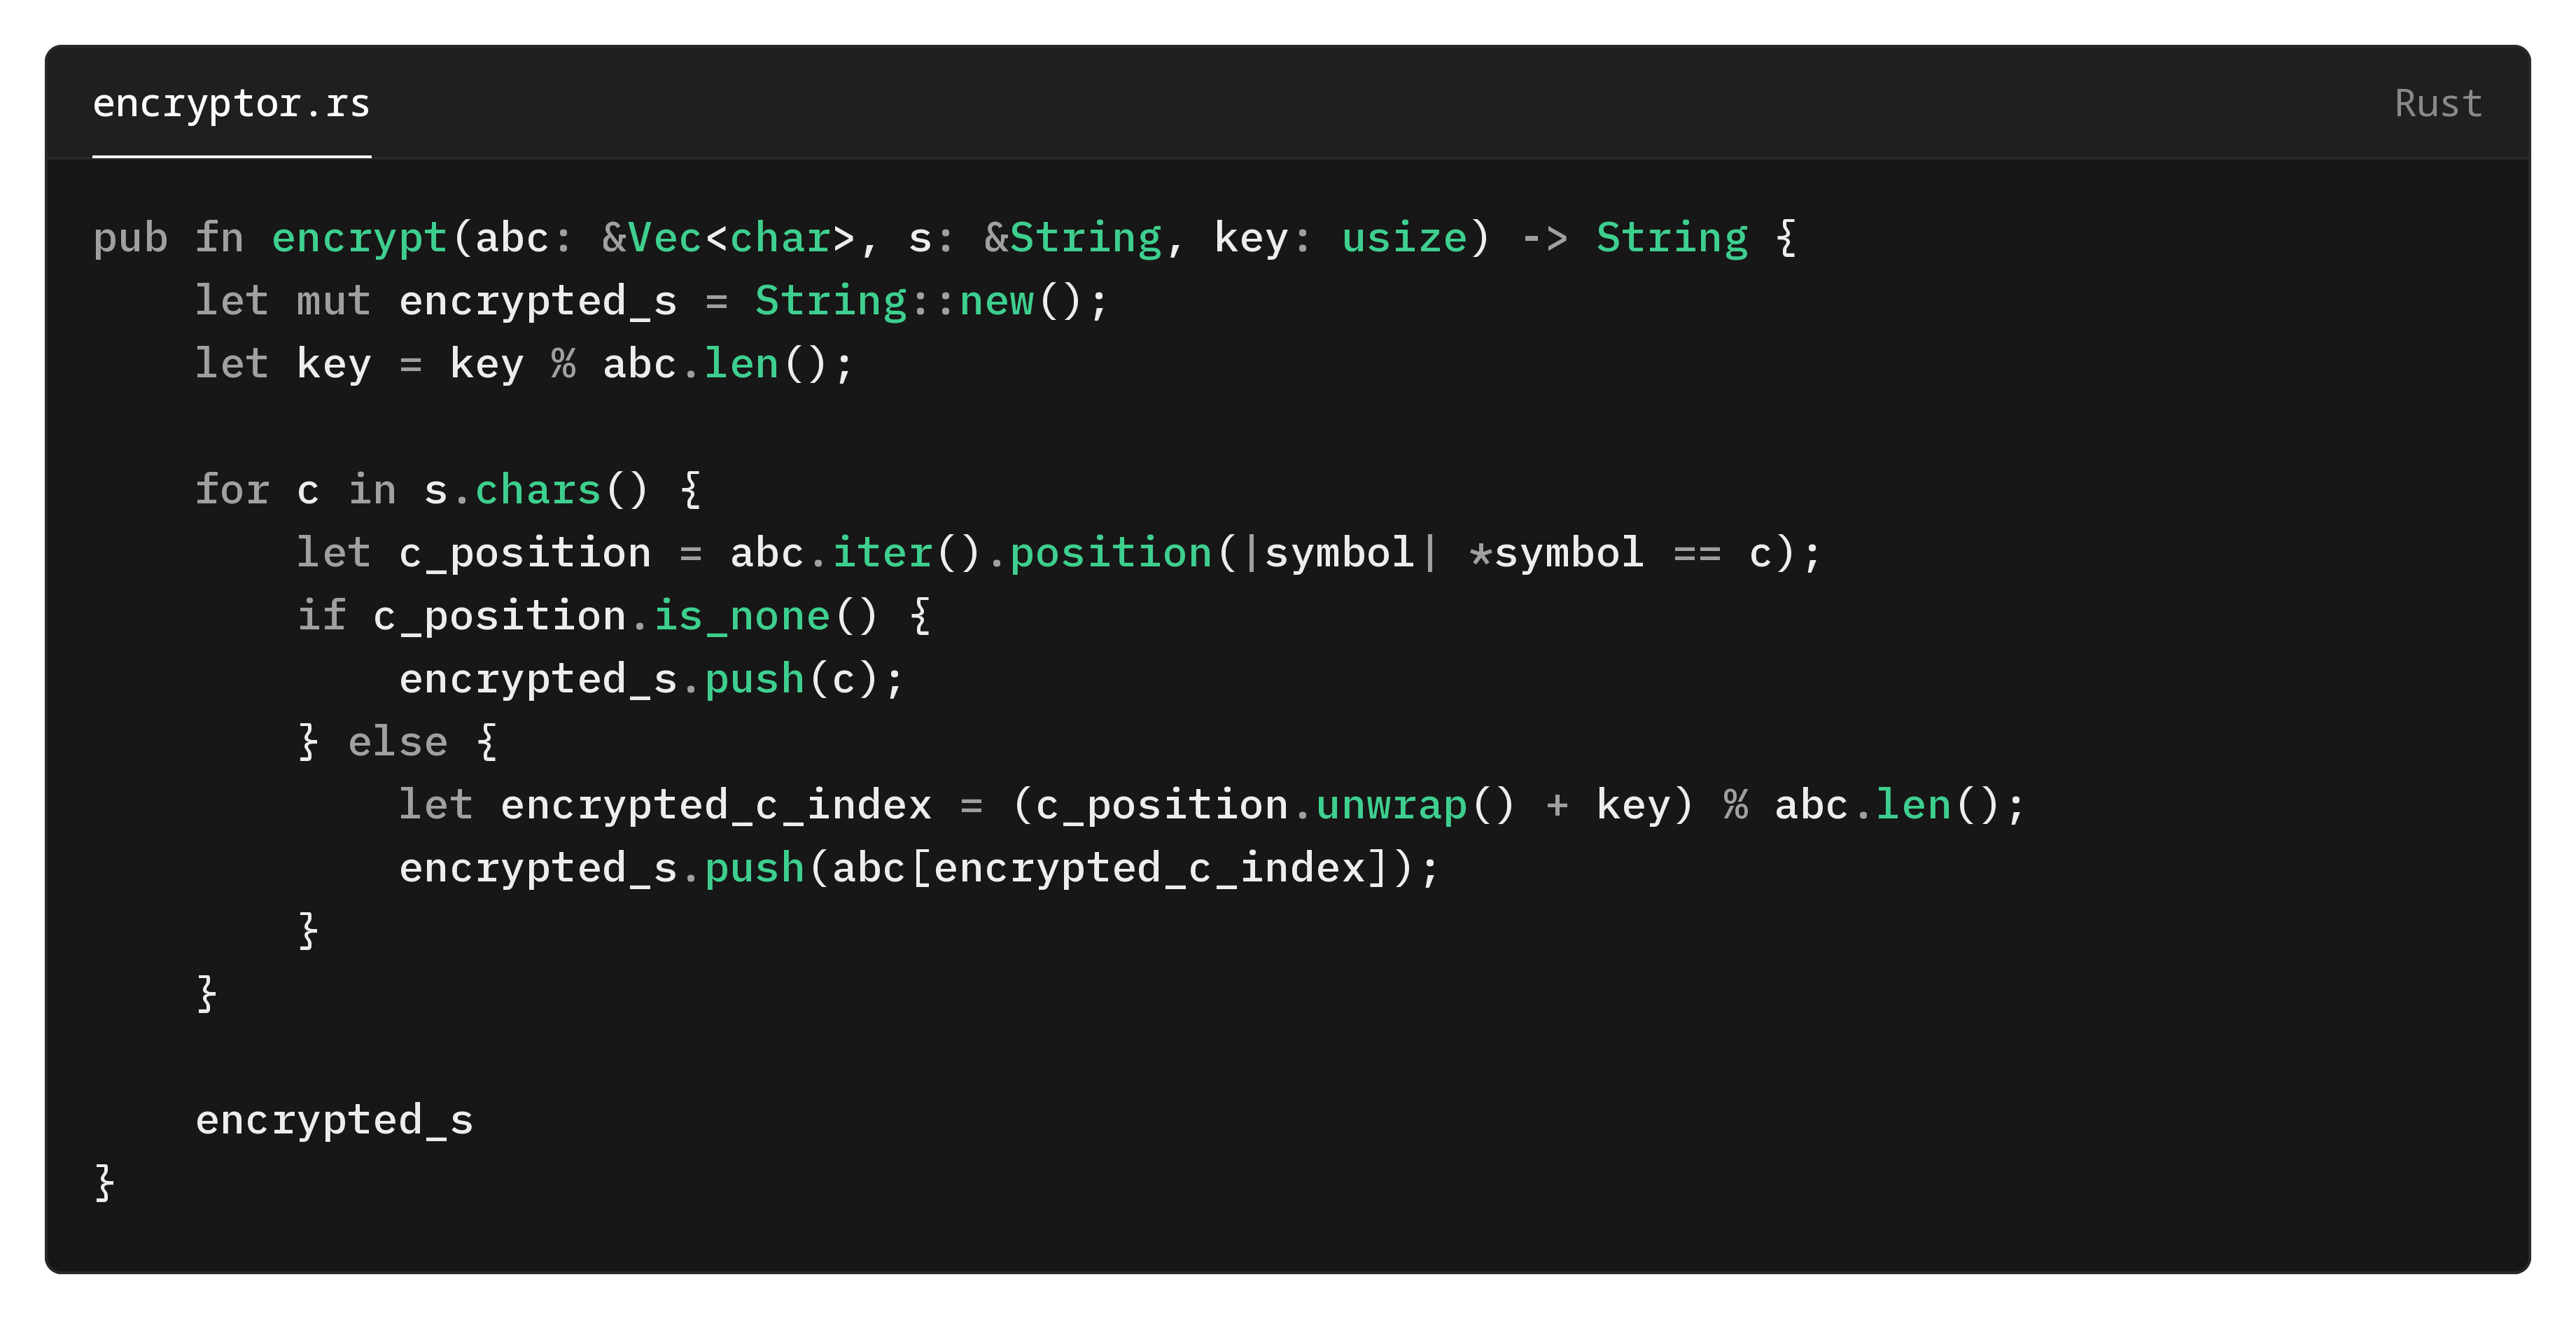
\includegraphics[width=1\textwidth]{images/caesars_cipher_encryptor.png}

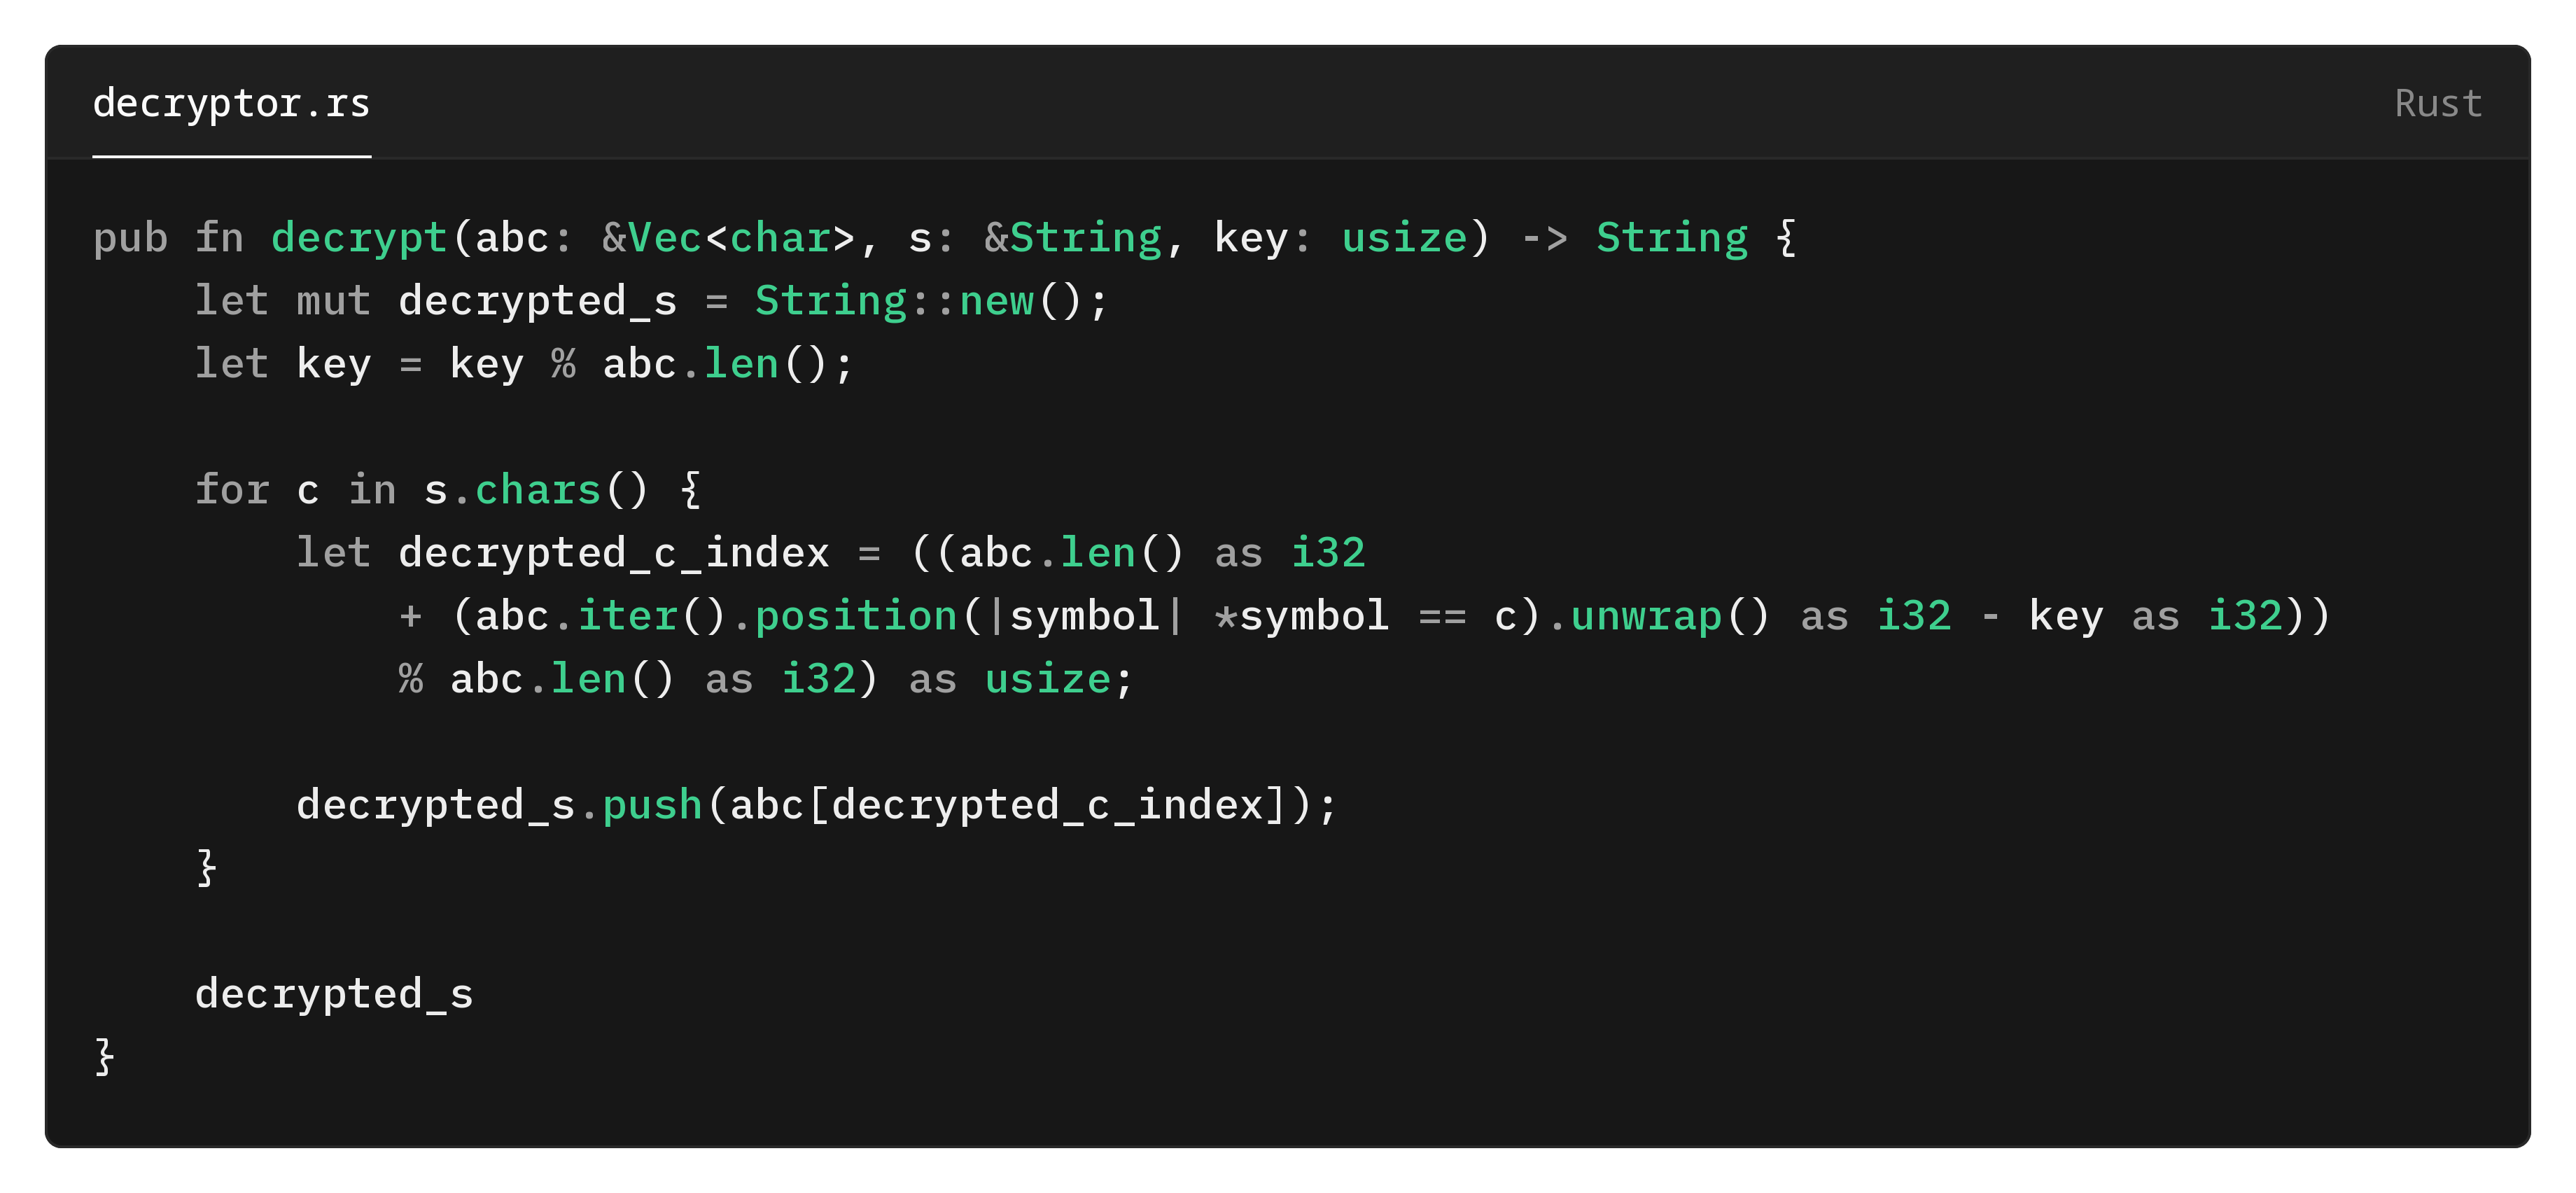
\includegraphics[width=1\textwidth]{images/caesars_cipher_decryptor.png}

\end{document}
